% !TEX root = ../../main.tex
\subsection{性能测试}

本节使用性能基准脚本对关键密码学操作和业务流程进行耗时测试。两组测试分别使用不同数据规模（第一组：10 用户、50 订单、1000 消息；第二组：20 用户、200 订单、6000 消息），结果如表~\ref{tab:perf_basic}所示，终端运行输出如图~\ref{fig:perf1}和图~\ref{fig:perf2}所示。

\begin{table}[H]
\centering
\caption{关键路径性能基准}
\label{tab:perf_basic}
\small
\setlength{\tabcolsep}{4pt}
\begin{tabular}{lrrrrrcrrrrr}
\hline
& \multicolumn{5}{c}{\textbf{第一组（50 订单，1000 消息）}} & & \multicolumn{5}{c}{\textbf{第二组（200 订单，6000 消息）}} \\
\cline{2-6} \cline{8-12}
\textbf{操作} & \textbf{avg} & \textbf{P95} & \textbf{max} & \textbf{N} & \textbf{单位} & & \textbf{avg} & \textbf{P95} & \textbf{max} & \textbf{N} & \textbf{单位} \\
\hline
Token 生成 & 1.199 & 1.488 & 1.862 & 50 & ms & & 1.181 & 1.421 & 1.888 & 200 & ms \\
Token 验证 & 1.133 & 1.374 & 1.683 & 50 & ms & & 1.130 & 1.379 & 4.007 & 200 & ms \\
SM4 加解密 & 0.547 & 0.607 & 1.641 & 1000 & ms & & 0.550 & 0.624 & 3.975 & 6000 & ms \\
消息写入+哈希 & 0.454 & 0.582 & 1.355 & 1000 & ms & & 0.461 & 0.577 & 4.242 & 6000 & ms \\
Merkle 快照 & 19.90 & 21.29 & 21.76 & 50 & ms & & 28.17 & 29.82 & 32.82 & 200 & ms \\
完整性验证 & 37.62 & 39.09 & 40.69 & 50 & ms & & 54.48 & 57.02 & 61.09 & 200 & ms \\
\hline
\end{tabular}
\end{table}

\begin{figure}[H]
\centering
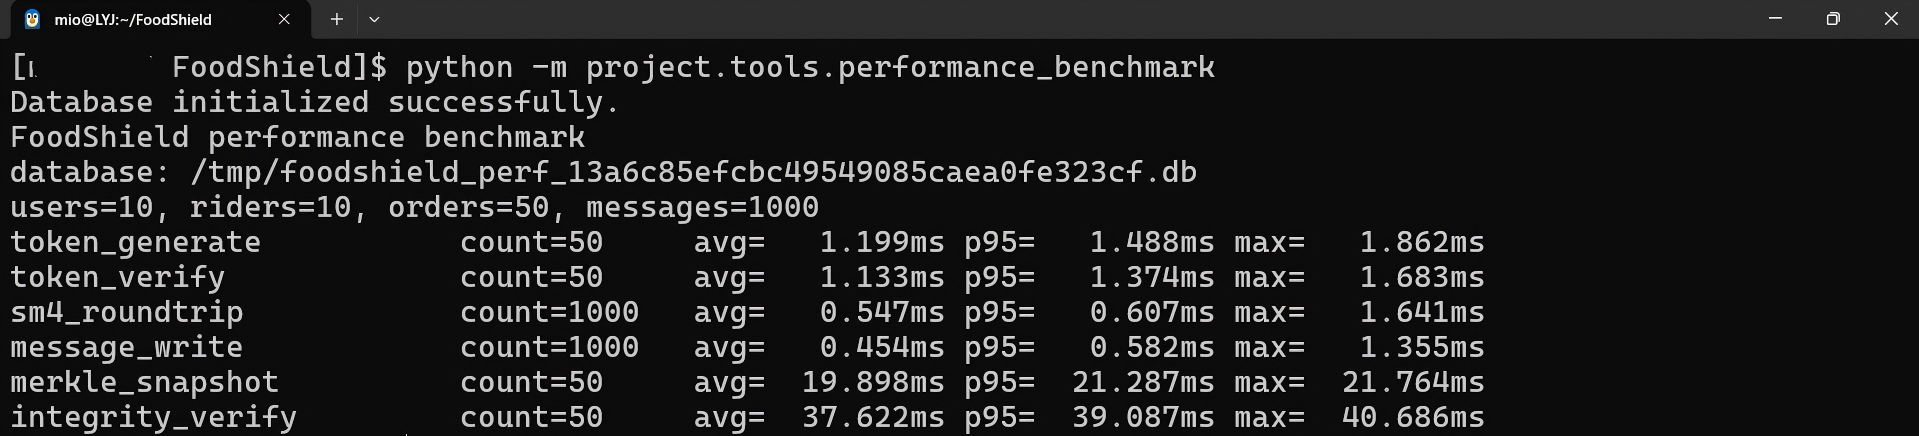
\includegraphics[width=0.95\textwidth]{content/chapter5/figure/perf.png}
\caption{第一组性能基准运行输出}
\label{fig:perf1}
\end{figure}

\begin{figure}[H]
\centering
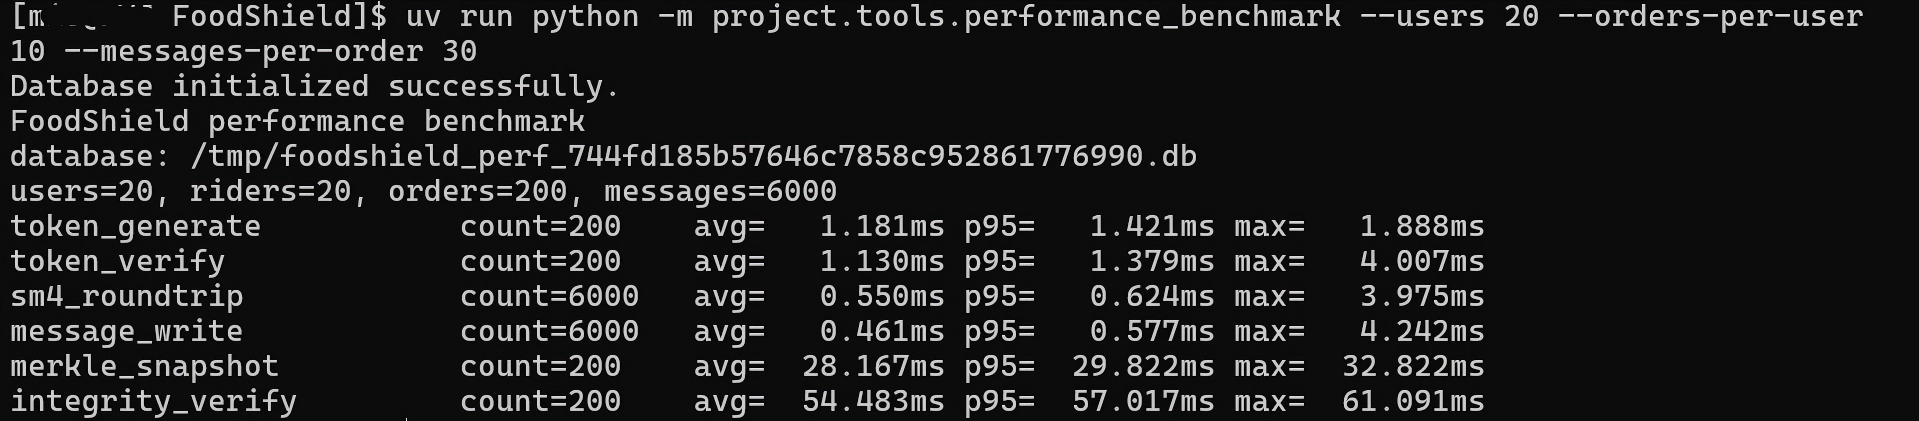
\includegraphics[width=0.95\textwidth]{content/chapter5/figure/perf2.png}
\caption{第二组性能基准运行输出}
\label{fig:perf2}
\end{figure}

\textbf{运行命令}：第一组 \texttt{python -m project.tools.performance\_benchmark}；第二组追加 \texttt{--users 20 --orders-per-user 10 --messages-per-order 30}。

\subsubsection*{性能分析}

\begin{enumerate}[label=\arabic*., leftmargin=2em]
\item \textbf{密码学操作耗时可控}：Token 生成与验证约 1.1--1.2\,ms，两组基本一致，说明 HMAC-SM3 耗时不受数据规模影响。SM4 加解密约 0.55\,ms，消息写入（含加密+哈希+SQLite INSERT）约 0.46\,ms，均满足实时通信要求。PID 生成同为 HMAC-SM3 操作，耗时与 Token 相当。

\item \textbf{Merkle 线性增长}：快照生成从 19.90\,ms（20 条/订单）增至 28.17\,ms（30 条/订单），每条消息约 0.94--0.99\,ms；完整性验证从 37.62\,ms 增至 54.48\,ms，每条约 1.82--1.88\,ms，均符合$O(n)$理论预期。

\item \textbf{瓶颈识别}：完整性验证是最耗时操作（需解密全部消息并重算哈希），但触发频率低（仅管理员主动验证或溯源前置校验时触发），不影响日常通信。日常关键路径（Token 验证 + SM4 加解密 + 消息写入）总耗时约 2\,ms。
\end{enumerate}
